L'algorithme de Dijkstra est un parcours en largeur d'un graphe \textbf{pondéré} et orienté. Il permet de calculer l'ensemble des plus courts chemins entre un sommet vers tous les autres sommets du graphe.

Pour modéliser le graphe, on utilisera une matrice d'adjacence $M$ pour laquelle $M_{ij}=w(i,j)$ et $w(i,j)$ représente le poids de l'arête de $i$ vers $j$. Lorsqu'il n'y a pas d'arc entre deux sommets, on aura $M_{ij}=\infty$.

\begin{exemple}~\\

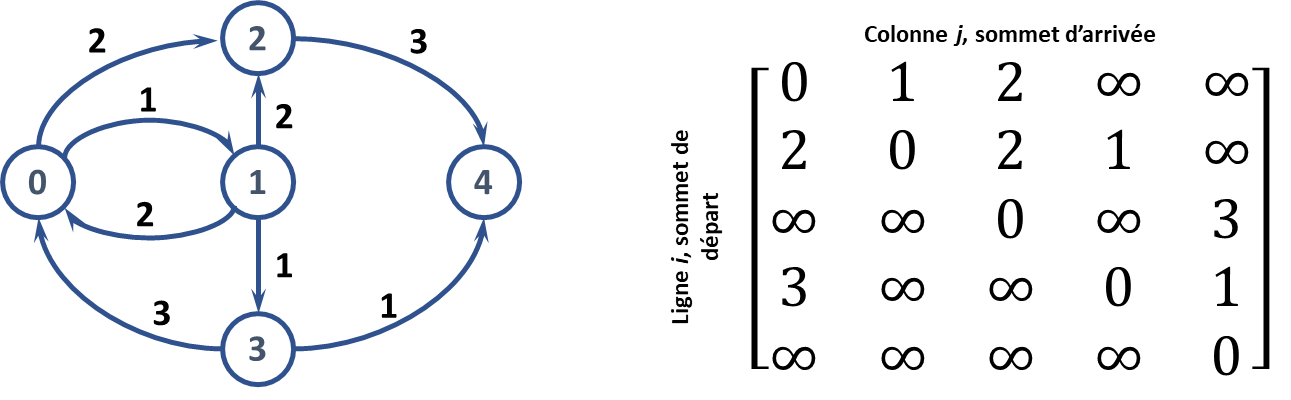
\includegraphics[width=.8\linewidth]{graphe_01}
\end{exemple}

\begin{defi}{Poids d'un chemin}
Soit un un graphe pondéré $G=\left(V, E, w\right)$ où $V$ désigne l'ensemble des sommets, $E$ l'ensemble des arêtes et 
$w$, la fonction poids définie par $w : E \rightarrow \mathbb{R}$ ($w(u, v)$ est le poids de l’arête de $u$ vers $v$).

On appelle poids du chemin $C$ et on note $w(C)$ la somme des poids des arêtes du chemin. 

Un chemin de $u\in V$ à $v\in V$ est un plus court chemin s'il n'existe pas de chemin de poids plus petit. 
\end{defi}